\chapter{Implementación de Prototipos Funcionales}
\label{chap:implementacion}

\section{Introducción a la Fase de Implementación}
La validación final de un modelo de machine learning no reside únicamente en sus métricas de rendimiento, sino en su capacidad para operar en un entorno práctico y funcional. Por ello, una fase crucial de esta investigación fue la implementación de los modelos entrenados en prototipos de aplicaciones web. Este capítulo detalla la arquitectura, el desarrollo y el proceso de despliegue de dos aplicaciones distintas, cada una encapsulando uno de los enfoques metodológicos explorados: el clasificador optimizado con algoritmos metaheurísticos y el modelo final basado en el ajuste fino de Transformers.

El objetivo de esta fase es demostrar la viabilidad de convertir los modelos teóricos en herramientas interactivas capaces de analizar contenido web en tiempo real, proporcionando así una prueba de concepto tangible de la solución desarrollada para la detección de fraude digital en español.

\section{Arquitectura General del Sistema}
Para asegurar la modularidad, portabilidad y escalabilidad, ambos prototipos se diseñaron siguiendo una arquitectura de microservicio web contenerizado. Esta arquitectura se compone de cuatro capas fundamentales que se describen a continuación.

\begin{itemize}
    \item \textbf{Frontend (Capa de Presentación):} Se desarrolló una interfaz de usuario limpia e intuitiva utilizando HTML5, CSS3 y JavaScript. Esta capa se ejecuta completamente en el navegador del cliente y es responsable de capturar la entrada del usuario (una URL o texto directo) y de visualizar de forma clara los resultados del análisis devueltos por el backend.
    
    \item \textbf{Backend (Capa de Lógica y API):} El corazón de la aplicación se construyó como una API RESTful utilizando \textbf{Flask}, un microframework de Python. Flask fue seleccionado por su ligereza, flexibilidad y su robusto ecosistema, ideal para servir modelos de machine learning. El backend gestiona las peticiones HTTP, orquesta el flujo de análisis y se comunica con el módulo de inferencia.
    
    \item \textbf{Módulo de Inferencia (Capa de IA):} Corresponde al modelo de machine learning entrenado. Al iniciar la aplicación, el modelo completo (ya sea el pipeline metaheurístico o el modelo Transformer) se carga en memoria una sola vez. Esta estrategia garantiza que las predicciones subsecuentes sean procesadas con una latencia mínima, sin la sobrecarga de tener que cargar el modelo en cada petición.
    
    \item \textbf{Contenerización (Capa de Despliegue):} La aplicación completa, junto con todas sus dependencias de Python y del sistema, se empaqueta en una imagen de contenedor utilizando \textbf{Docker}. El proceso es gestionado por un archivo \texttt{docker-compose.yml}, que permite construir y ejecutar la aplicación en un entorno aislado y reproducible con un solo comando. Esto elimina los problemas de compatibilidad entre diferentes máquinas y simplifica drásticamente el despliegue.
\end{itemize}

\section{Prototipo 1: Analizador Basado en Metaheurísticas}
El primer prototipo se desarrolló para servir los modelos optimizados con los algoritmos metaheurísticos (Recocido Simulado, Búsqueda Dispersa, etc.). Esta implementación sirvió como una valiosa prueba de concepto y como una base de comparación para el modelo Transformer final.

\subsection{Componentes del Modelo}
El ``modelo'' en este enfoque no es un único archivo, sino un pipeline de preprocesamiento y clasificación compuesto por cinco artefactos distintos, todos ellos guardados en la carpeta \texttt{app/modelo\_recocido/}:
\begin{itemize}
    \item \texttt{vectorizer.joblib:} El objeto \texttt{TfidfVectorizer} entrenado, responsable de convertir texto nuevo al formato TF-IDF.
    \item \texttt{selector\_caracteristicas.joblib:} El objeto \texttt{SelectPercentile} que aplica la reducción de dimensionalidad, seleccionando solo las características más relevantes.
    \item \texttt{modelo\_recocido\_solucion.npy:} Array de NumPy que define los índices de las características a utilizar.
    \item \texttt{modelo\_recocido\_pesos.npy:} Array de NumPy con los pesos optimizados por el algoritmo.
    \item \texttt{modelo\_recocido\_umbrales.npy:} Array de NumPy con los umbrales de activación para cada característica.
\end{itemize}

\subsection{Flujo de Inferencia}
El archivo \texttt{main.py} de esta aplicación orquesta un flujo de inferencia de múltiples pasos para cada URL recibida:
\begin{enumerate}
    \item \textbf{Scraping y Limpieza:} Se extrae el texto de la URL y se aplica la misma función de limpieza de texto utilizada durante la creación del corpus.
    \item \textbf{Vectorización:} El texto limpio se transforma en un vector numérico utilizando el \texttt{vectorizer} cargado.
    \item \textbf{Selección de Características:} El vector se pasa a través del \texttt{selector} para reducir su dimensionalidad.
    \item \textbf{Clasificación:} Se aplican los \texttt{pesos} y \texttt{umbrales} sobre el vector reducido para calcular una probabilidad final y emitir un veredicto.
\end{enumerate}

\section{Prototipo 2: Analizador Basado en Modelos Transformer (Versión Final)}
El segundo prototipo, que representa la culminación del proyecto, implementa el modelo \texttt{DistilBERT} de mayor rendimiento. Esta aplicación demostró ser la más fiable y precisa de las dos.

\subsection{Componentes del Modelo}
Este modelo se guarda en el formato estándar de Hugging Face en la carpeta \texttt{app/modelo\_final\_distilbert\_es/}. Este formato encapsula de manera eficiente todos los componentes necesarios:
\begin{itemize}
    \item \texttt{tf\_model.h5:} Contiene la arquitectura y los **pesos del modelo** ajustados durante el fine-tuning.
    \item \texttt{config.json:} Archivo de configuración que describe la arquitectura del modelo.
    \item \texttt{tokenizer.json, vocab.txt, etc.:} Archivos que definen el **tokenizador** exacto, garantizando un preprocesamiento consistente.
\end{itemize}

\subsection{Flujo de Inferencia}
El proceso de inferencia con el modelo Transformer es notablemente más directo y potente:
\begin{enumerate}
    \item \textbf{Scraping y Combinación:} Se extrae el título y el texto de la URL y se combinan en el formato \texttt{"título [SEP] texto"}.
    \item \textbf{Tokenización:} Se utiliza el \texttt{AutoTokenizer} cargado para convertir el texto en los tensores de entrada que el modelo espera.
    \item \textbf{Predicción:} Los tensores se pasan al modelo \texttt{TFAutoModelForSequenceClassification}, que procesa la entrada a través de sus capas de atención y devuelve los \textit{logits} de salida.
    \item \textbf{Cálculo de Probabilidad:} Se aplica una función Softmax a los \textit{logits} para obtener las probabilidades finales de cada clase (FALSO/REAL) y se emite el veredicto.
\end{enumerate}

\section{Interfaz de Usuario y Casos de Uso}
Ambos prototipos comparten una interfaz de usuario común, definida en el archivo \texttt{index.html}, que permite una interacción fluida y proporciona un análisis detallado. A continuación se muestran capturas de pantalla de la aplicación final en funcionamiento.

\subsection{Caso de Uso 1: Detección de una Noticia Real}
En la Figura \ref{fig:app_real}, se introduce la URL de una noticia de una fuente verificada. La aplicación extrae correctamente el contenido y, basándose en el análisis del modelo Transformer, emite un veredicto de **REAL** con una alta confianza, demostrando la capacidad del sistema para identificar texto legítimo.

\begin{figure}[htbp]
    \centering
    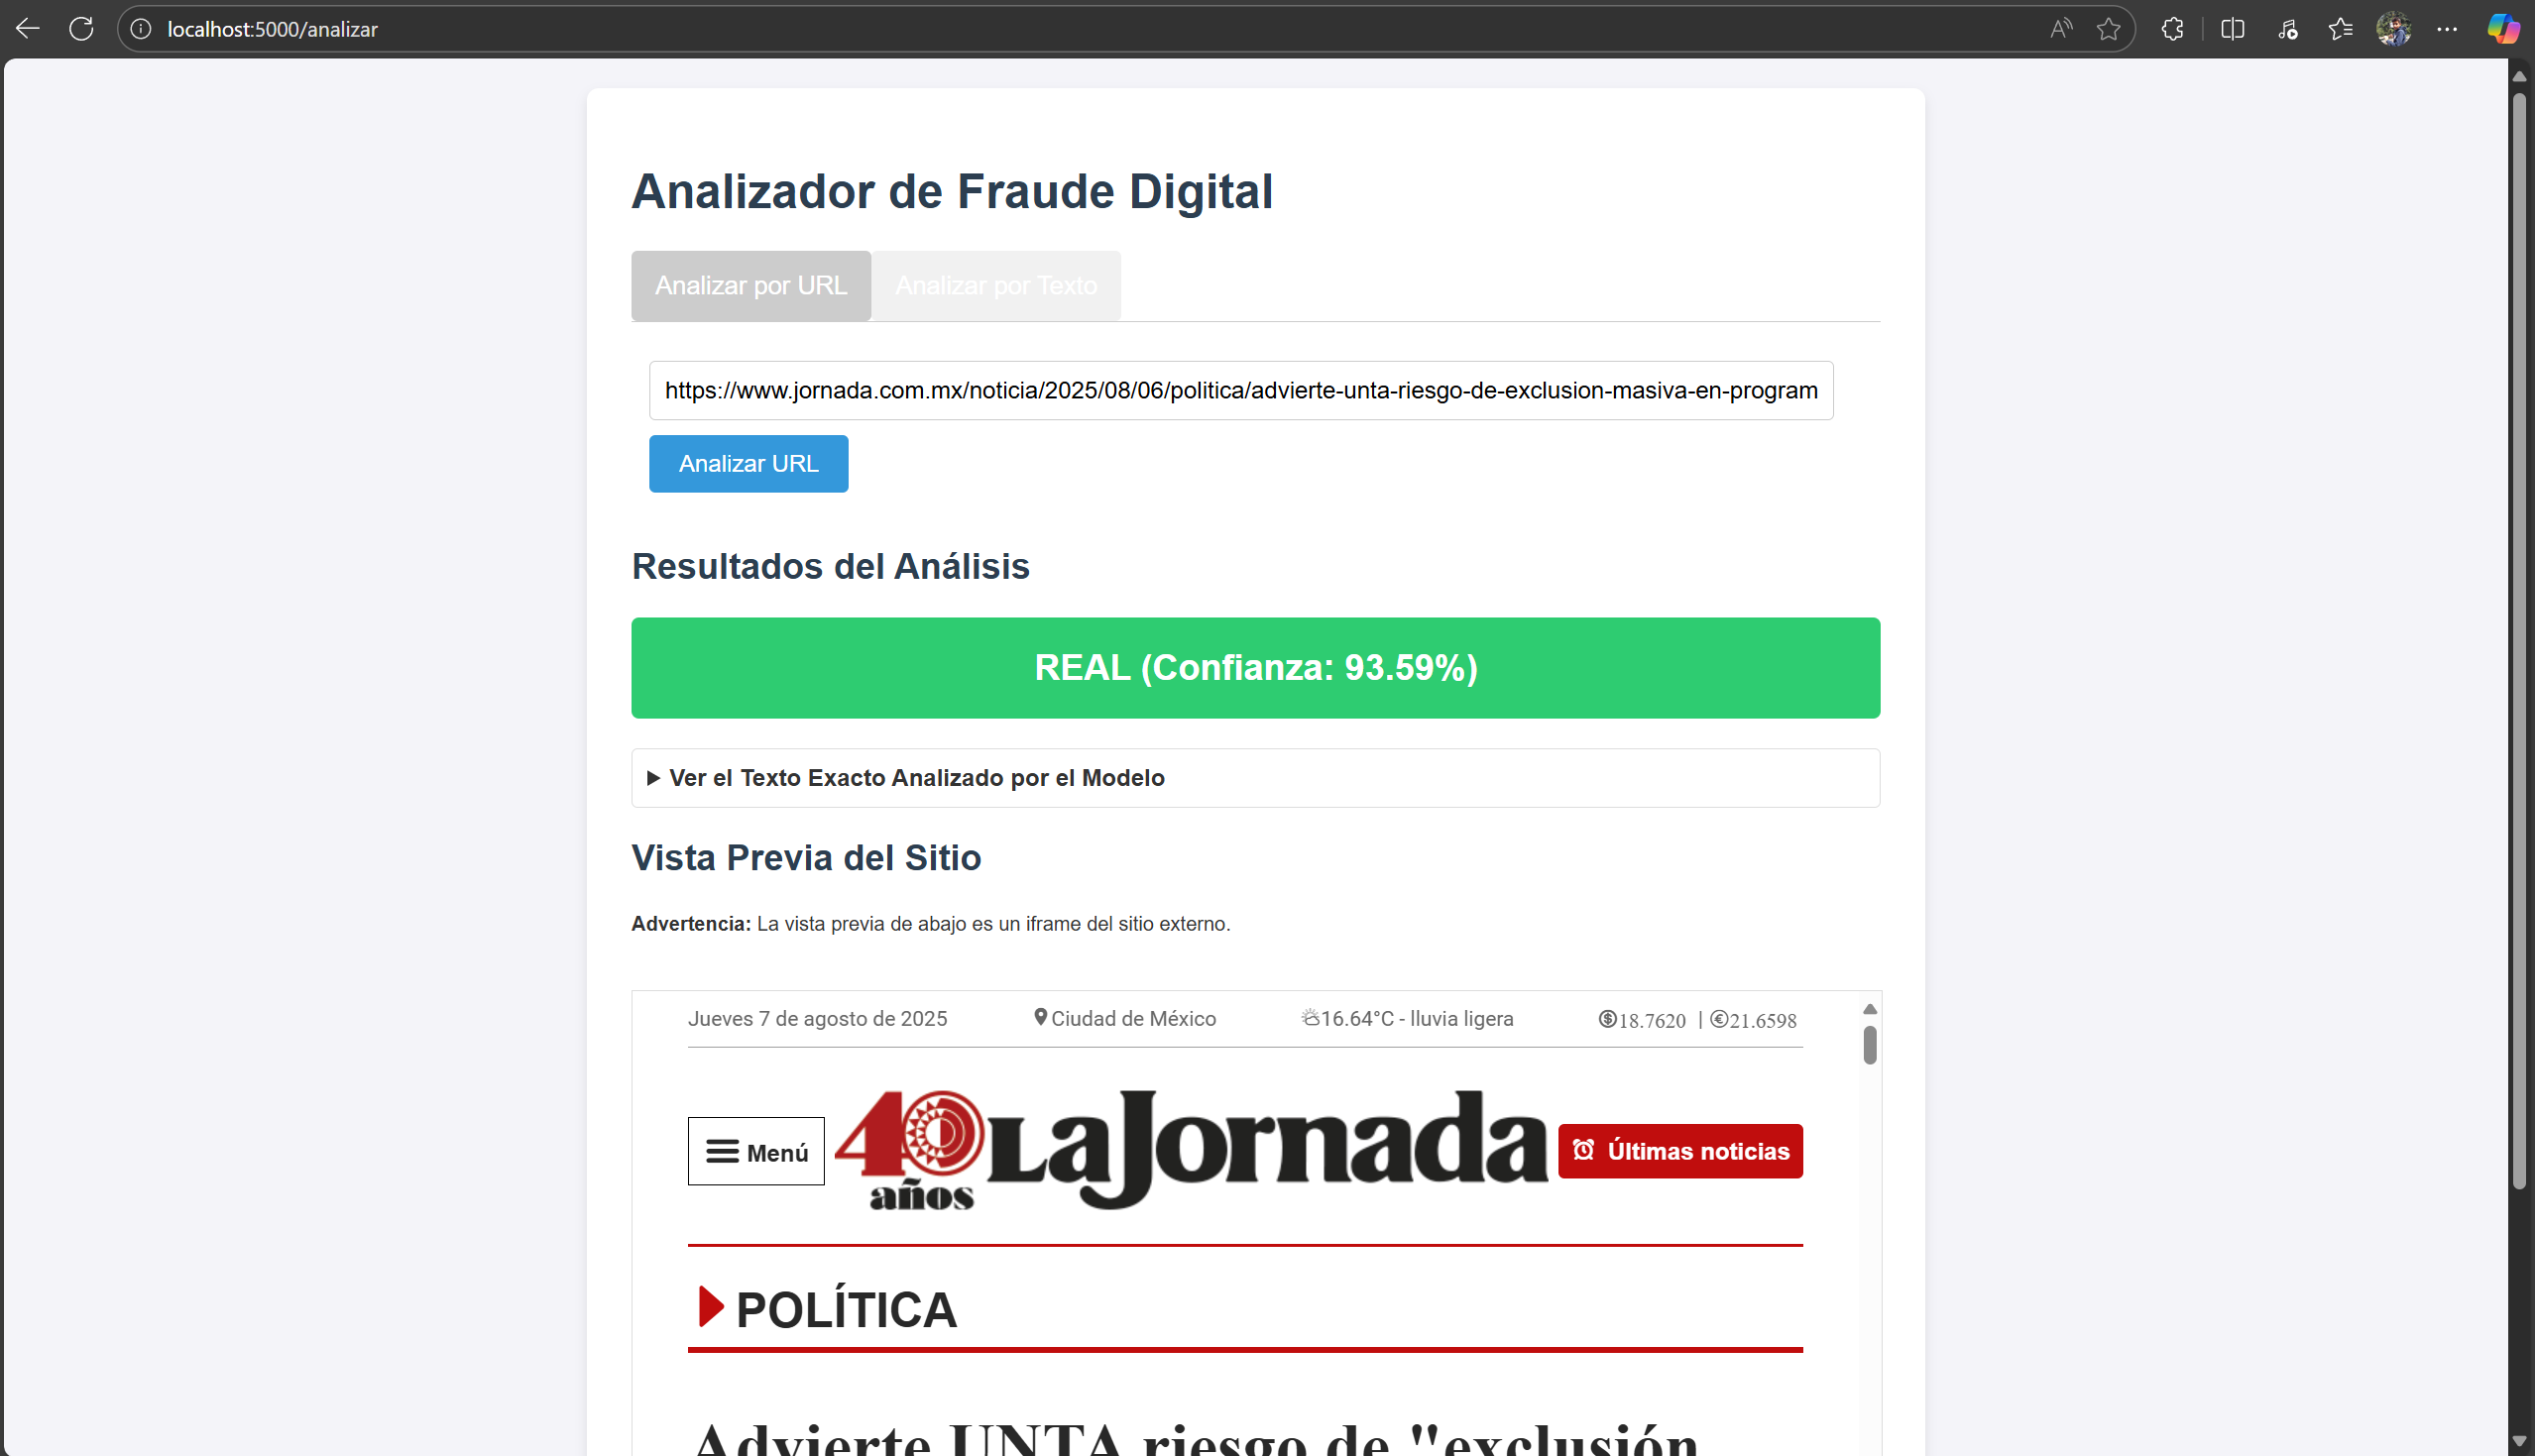
\includegraphics[width=0.9\textwidth]{Imagenes/app_real.png} % Reemplaza con la ruta a tu captura de pantalla
    \caption{Captura de pantalla de la aplicación analizando una noticia real.}
    \label{fig:app_real}
\end{figure}

\subsection{Caso de Uso 2: Detección de una Página con Contenido Engañoso}
La Figura \ref{fig:app_falsa1} muestra el análisis de una URL con contenido engañoso. El modelo de lenguaje identifica patrones en la redacción (exageraciones, estilo, etc.) que son inconsistentes con el periodismo real y la clasifica correctamente como **FALSA** con un alto grado de confianza.

\begin{figure}[htbp]
    \centering
    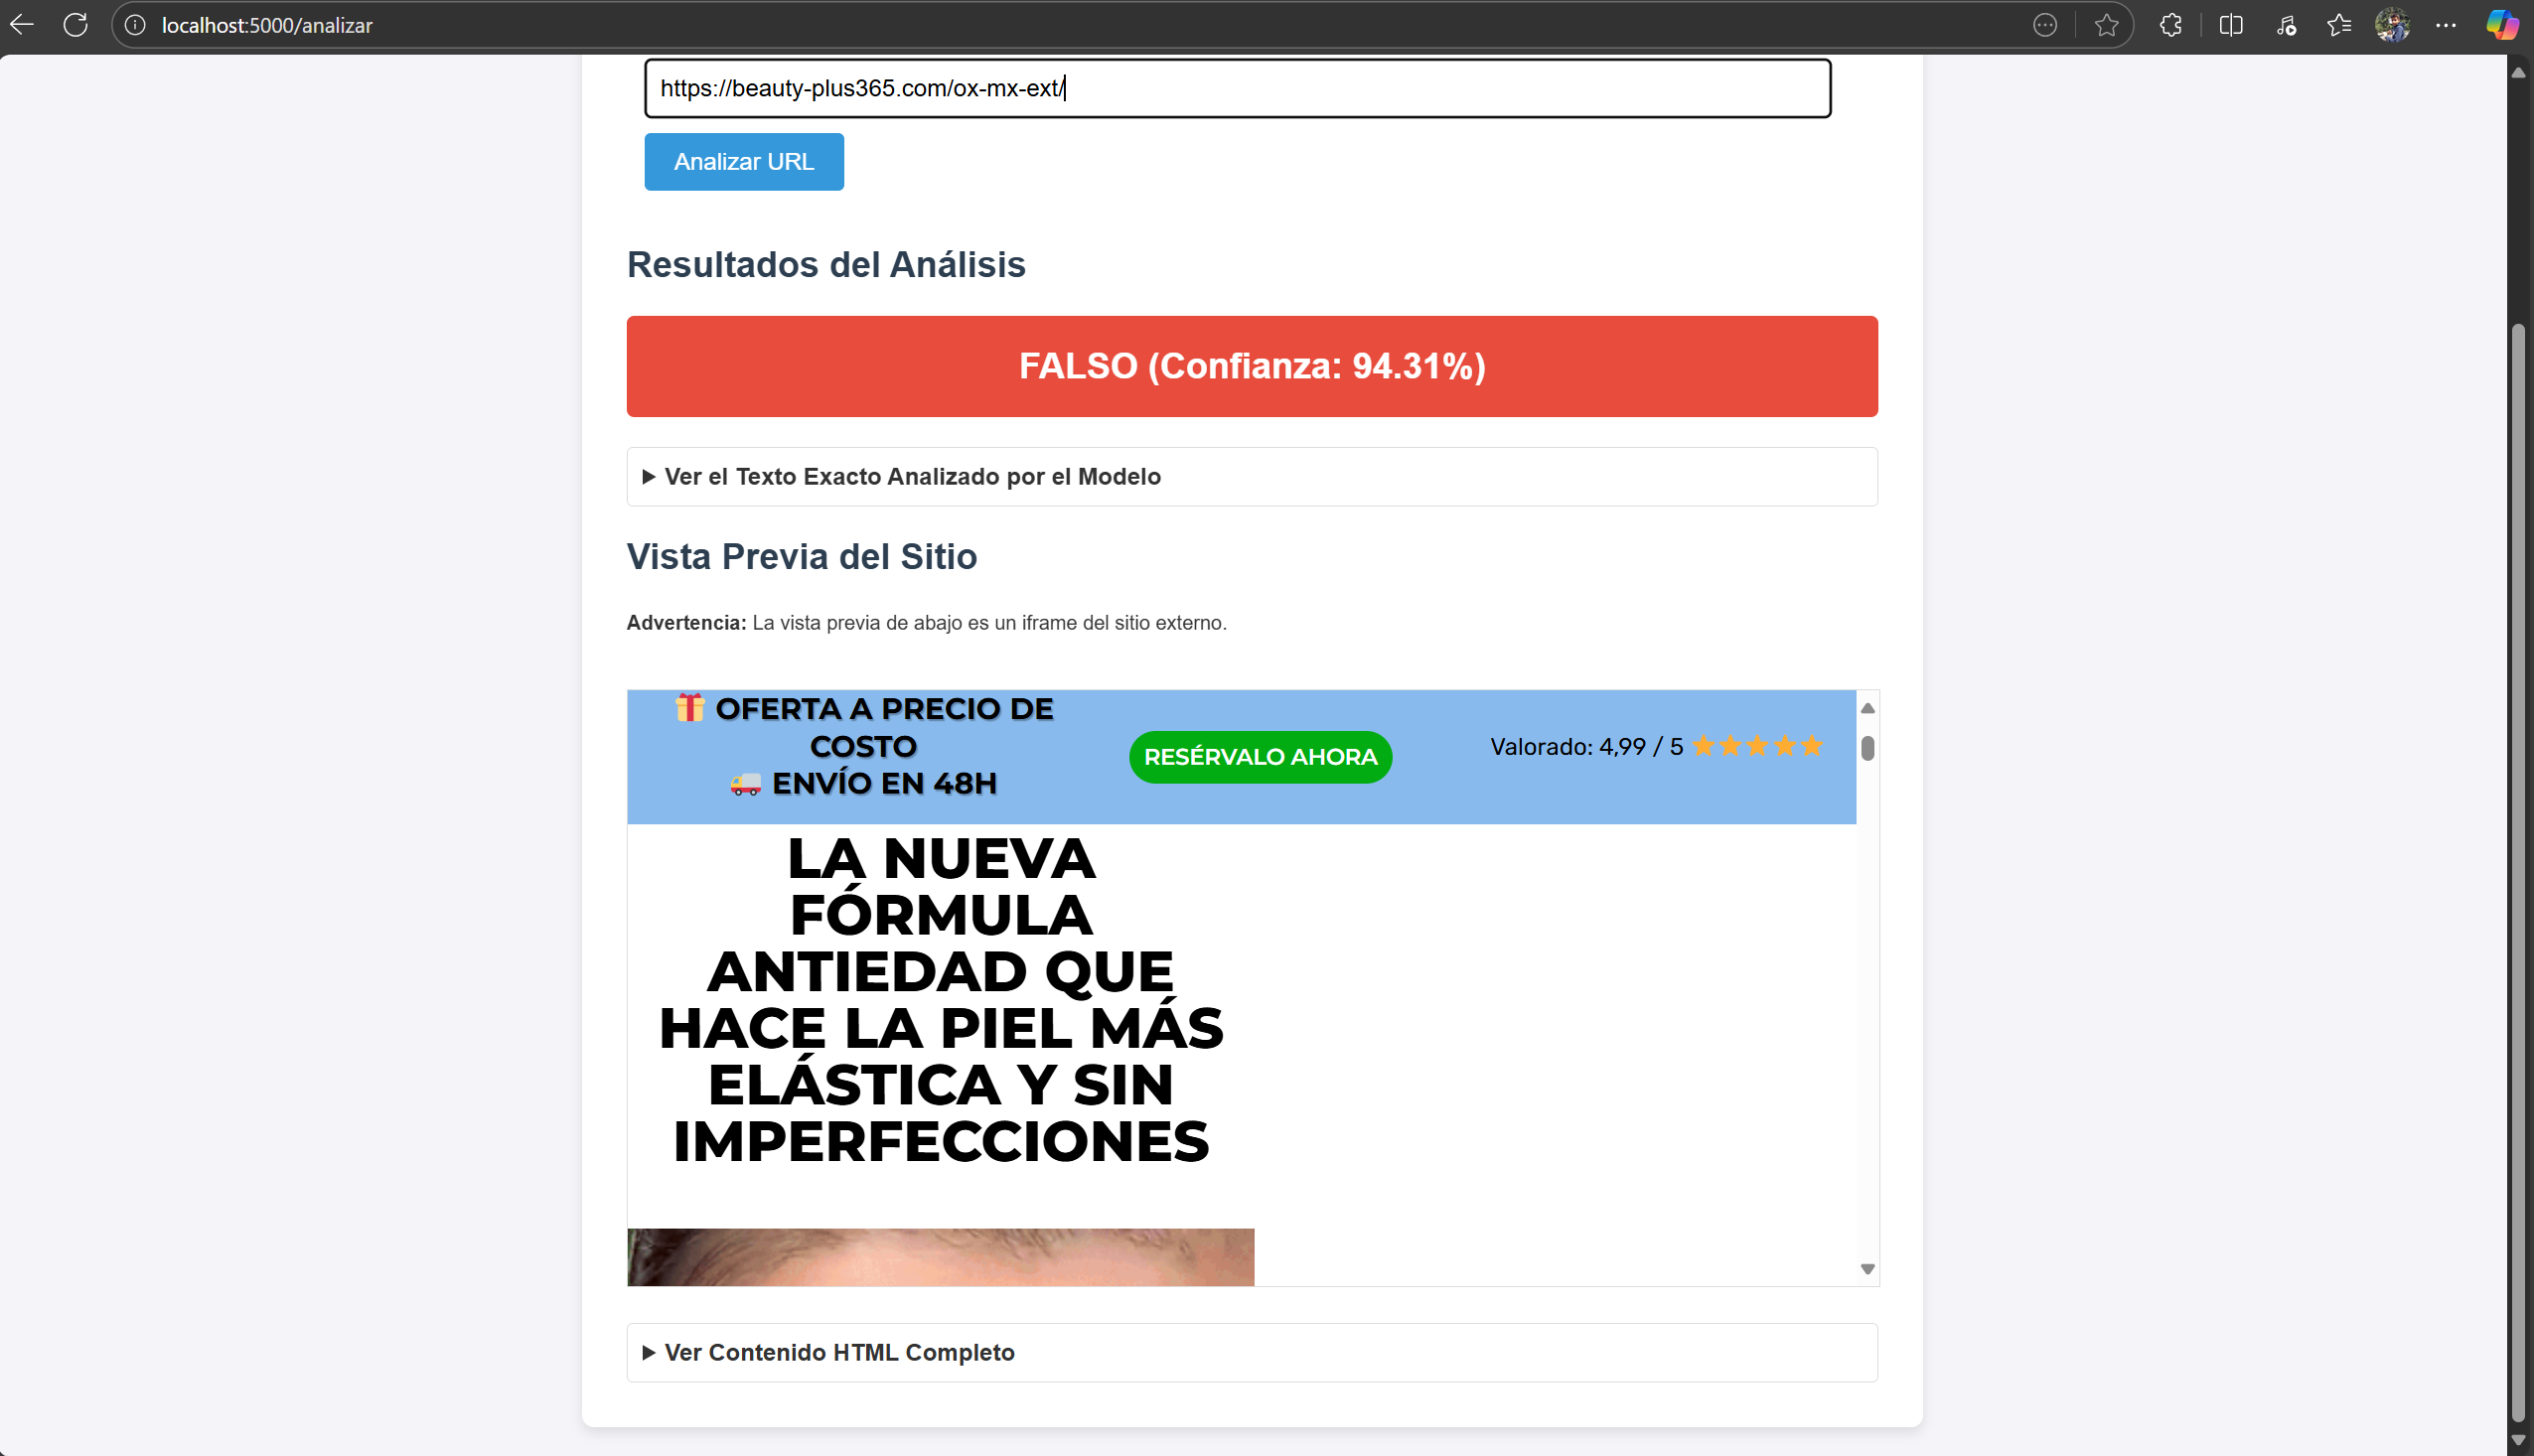
\includegraphics[width=0.9\textwidth]{Imagenes/app_falsa1.png} % Reemplaza con la ruta a tu captura de pantalla
    \caption{Captura de pantalla de la aplicación detectando una noticia falsa basada en su contenido.}
    \label{fig:app_falsa1}
\end{figure}

\subsection{Caso de Uso 3: Detección de una Página Fraudulenta}
Finalmente, la Figura \ref{fig:app_falsa2} ilustra un caso donde se introduce una URL de una página de inversión fraudulenta. El modelo, habiendo sido entrenado con ejemplos similares, detecta el lenguaje de urgencia y las promesas poco realistas, emitiendo un veredicto de **FALSO** con una confianza casi del 100\%, demostrando su utilidad como herramienta de prevención de fraude digital.

\begin{figure}[htbp]
    \centering
    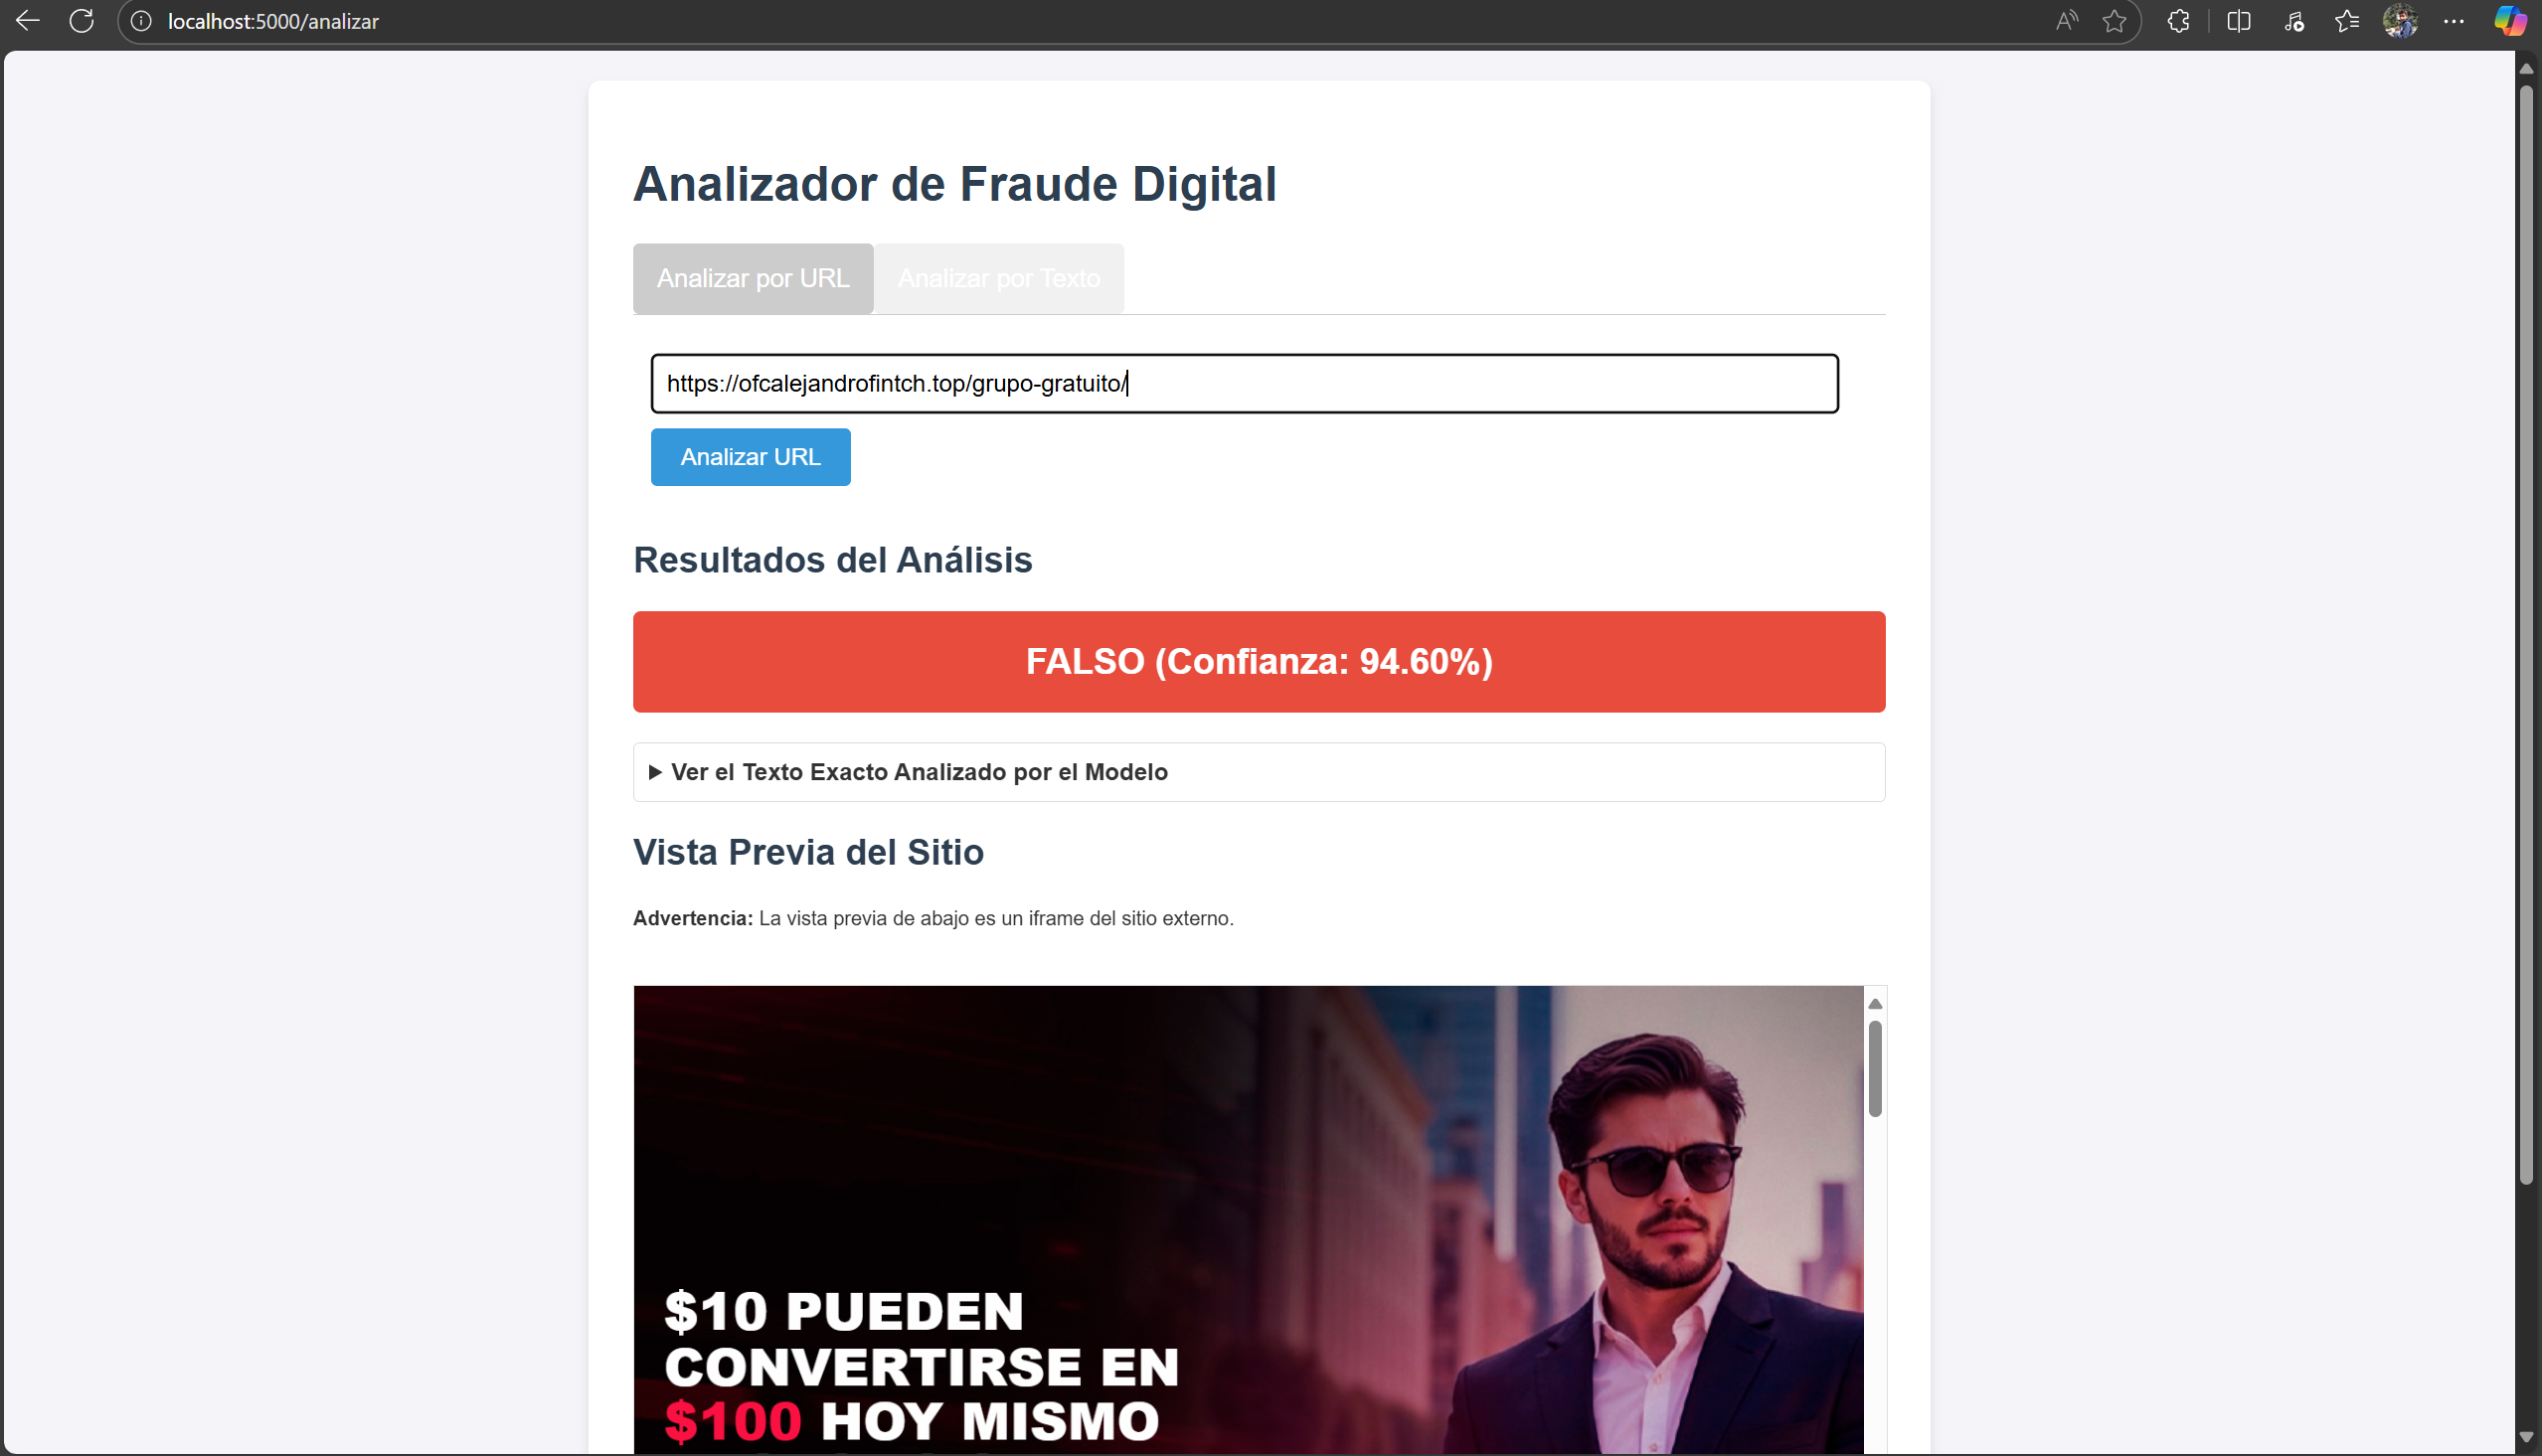
\includegraphics[width=0.9\textwidth]{Imagenes/app_falsa2.png} % Reemplaza con la ruta a tu captura de pantalla
    \caption{Captura de pantalla de la aplicación detectando una página de fraude digital.}
    \label{fig:app_falsa2}
\end{figure}